In order to achieve better discrimination between the Higgs boson signal and the SM backgrounds
compared to simple cuts we employ a Matrix Element technique. 
Compared to the selections applied in the $M_T$ analysis described in Section~\ref{sec:anal_mt}, we 
apply the same Higgs dependent selections except for the $M_T$ window cuts. 


This method has been previously used in precision
measurements of the top quark mass \cite{ref:CDFTopMass,ref:D0TopMass} and cross-section, 
diboson cross section \cite{ref:CDFDiboson},
as well as searches for single top \cite{ref:CDFSingleTop,ref:D0SingleTop} 
and Higgs boson production at the Tevatron \cite{ref:CDFHiggs,ref:D0Higgs}.
This method has also been validated in the $H\to WW\to 2\ell2\nu$ analysis as 
a cross-check to the BDT based analysis~\cite{HWW2011AN}. 

The Matrix Element method works by calculating the probability for each recorded
event to originate from a specific physics process.
This is done by comparing the differential cross sections predicted by Matrix Element 
calculations for the signal and background processes given the kinematic observables
on an event-by-event basis.
The discriminating power arises because the differential cross sections for 
signal and background events are largest in different regions of the available
kinematic phase space. 
One complication of the Higgs to $\ZZ\to 2\ell2\nu$ final state is that it is not fully 
reconstructed, with two neutrinos in the final state. 
Information about the $z$-components of the neutrino momenta as well as the individual 
neutrino transverse components are missing. It is therefore necessary to integrate 
over these unknown quantities, which we perform using the importance sampling 
integration method.
The Matrix Element functions used in the determination of the differential cross sections
for this analysis are obtained from  MCFM~\cite{mcfm}. While MCFM 
provides both leading order (LO) and next-to leading (NLO) cross-section calculations for 
all relevant background and Higgs processes in $pp$ collisions, only the
LO is currently used.

The probabilities for all processes under consideration are combined 
to construct a single discriminant, called the Likelihood Ratio ($LR$).  
To construct the optimal discriminant, one should calculate 
event probabilities for all of the background processes. In reality, however, having 
probabilities for the signal hypothesis and the main backgrounds is sufficient for the 
desired level of discrimination. In this analysis we calculate event probabilities 
for gluon fusion Higgs boson production ($ggH$), electroweak $q\bar{q}\rightarrow ZZ\to 2\ell2\nu$ 
and $q\bar{q}\rightarrow WZ\to l\nu2\ell$ processes and the $q\bar{q}\rightarrow WW$ processes. 


\subsubsection{Event Probability Calculation}

In the Matrix Element technique we calculate a probability for each event assuming a
certain hypothesis.  The probability is denoted by $P(x_{obs};\alpha)$,
where $\alpha$ is a set of physics 
parameters of the specific model and $x_{obs}$ are the measured kinematic quantities.
In the case of Standard Model Higgs Boson production,
 $\alpha$ is $(m_H, \Gamma_H)$, where  $m_H$ is the Higgs mass 
and $\Gamma_H$ is the Higgs width. There are eight observables, $x_{obs}$, representing all the 
lepton kinematic information: lepton momenta $\vec{l}^+$, $\vec{l}^-$ and missing 
transverse momentum, \met$_x$ and \met$_y$.

It should be noted that additional information such as the number of jets
produced and the total visible energy might further differentiate the Higgs signal from SM
$WW$ production,
but they can suffer from significant  QCD uncertainties. For this reason we 
deliberately do not use hadronic information at all but use
only the kinematic information from the leptons and the missing $E_T$.

The event probability density is given by
\begin{equation}
P(x_{obs};\alpha) =
 {1 \over < \sigma(\alpha) > }
 \int \frac {d \sigma_{0} (y;\alpha) }{ dy }
 \epsilon (y) G(x_{obs},y) dy,  
\label{eqn:EvtProb}  
\end{equation}
where $y$ denotes the true values of the observables,
$d \sigma_{LO} \over  dy$ is the  parton-level differential cross-section differential
in those observables, $\epsilon(y)$ is the detector acceptance and efficiency function
and $G(x_{obs},y)$ is the transfer function between the true and measured values of the
observables, representing the detector resolution.
Equation (\ref{eqn:EvtProb}) integrates over all possible true values of the
observables, $y$, consistent with the measured quantities $x_{obs}$.
The constant $<\sigma(\alpha)>$ normalizes the total event probability to unity
%, i.e.
%\begin{equation}
%\int_{x_{obs}\in V_{acceptance}} { P ( x_{obs}; \alpha)  d x_{obs} } = 1.
%\end{equation}
and is equal to the LO cross-section ($\sigma_{LO}$) times the acceptance.
%One complication of the Higgs to $WW$ leptonic final state is that it is not fully 
%reconstructed. Information about $z$-components of neutrino momenta as well as individual 
%neutrino transverse components are missing. It is, therefore, necessary to integrate 
%over these unknown quantities which we do using importance sampling integration method.

%\subsubsection{Efficiency Function}
The efficiency function is the probability for a parton-level object with momentum 
$p$ to be reconstructed as a lepton with momentum $q$. In the calculation of the event 
probabilities we assume that the parton level lepton momentum is equal to the reconstructed 
momentum. The lepton efficiency is parameterized as a function of transverse momentum and 
pseudo-rapidity and extracted from $WW$ Monte Carlo. 
%Figure~\ref{fig:lepeff_gen} shows the 
%one dimensional projection of the efficiency as a function of the lepton $\eta$ and $\pt$. 
%A scale factor to account for
%differences between data and Monte Carlo can be calculated using a tag-and-probe analysis 
%and applied when calculating event probabilities for data events. 
Note that the efficiency function in Equation~\ref{eqn:EvtProb} can be factorized out of
the integral when calculating event probabilities.
%The efficiency function in Equation~\ref{eqn:EvtProb} can be pulled out from 
%the integral when calculating event probabilities, for example in the case of $WW$ process:
%\begin{eqnarray}
%\begin{array}{lcl}
%P_{WW}(x_{obs};\alpha) & = &
% \frac{\epsilon (\eta_{1,obs})\epsilon (\eta_{2,obs})}{ < \sigma_{WW} > }
% \int \frac {d \sigma_{WW} (y;\alpha) }{ dy }
%  G(x_{obs},y) dy. \\
%\end{array} 
%\end{eqnarray}

%%%%%%%%%%%%%%%%%%%%%%%%%%%%%%
%\begin{figure}[!htbp]
%\begin{center}
%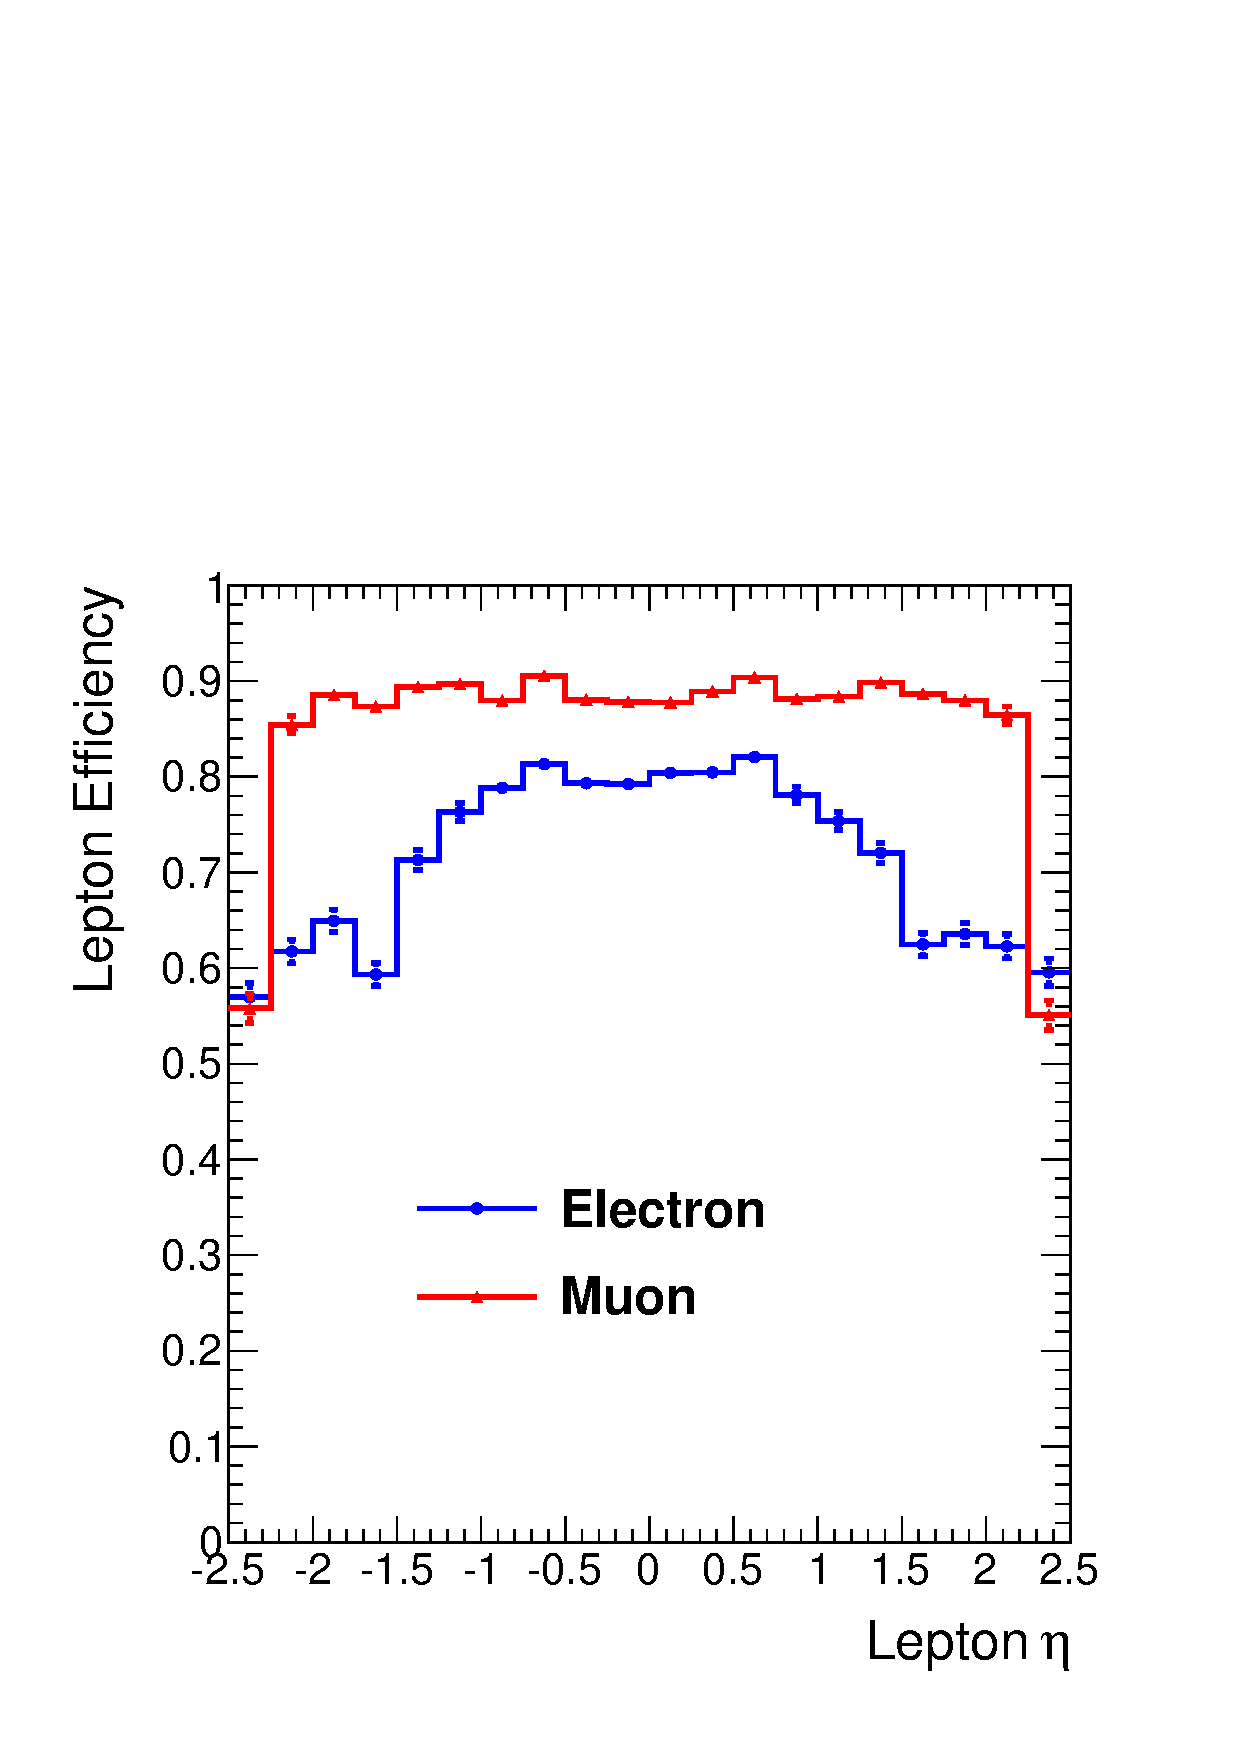
\includegraphics[width=0.4\textwidth]{figures/lepton_eff_Eta.pdf}
%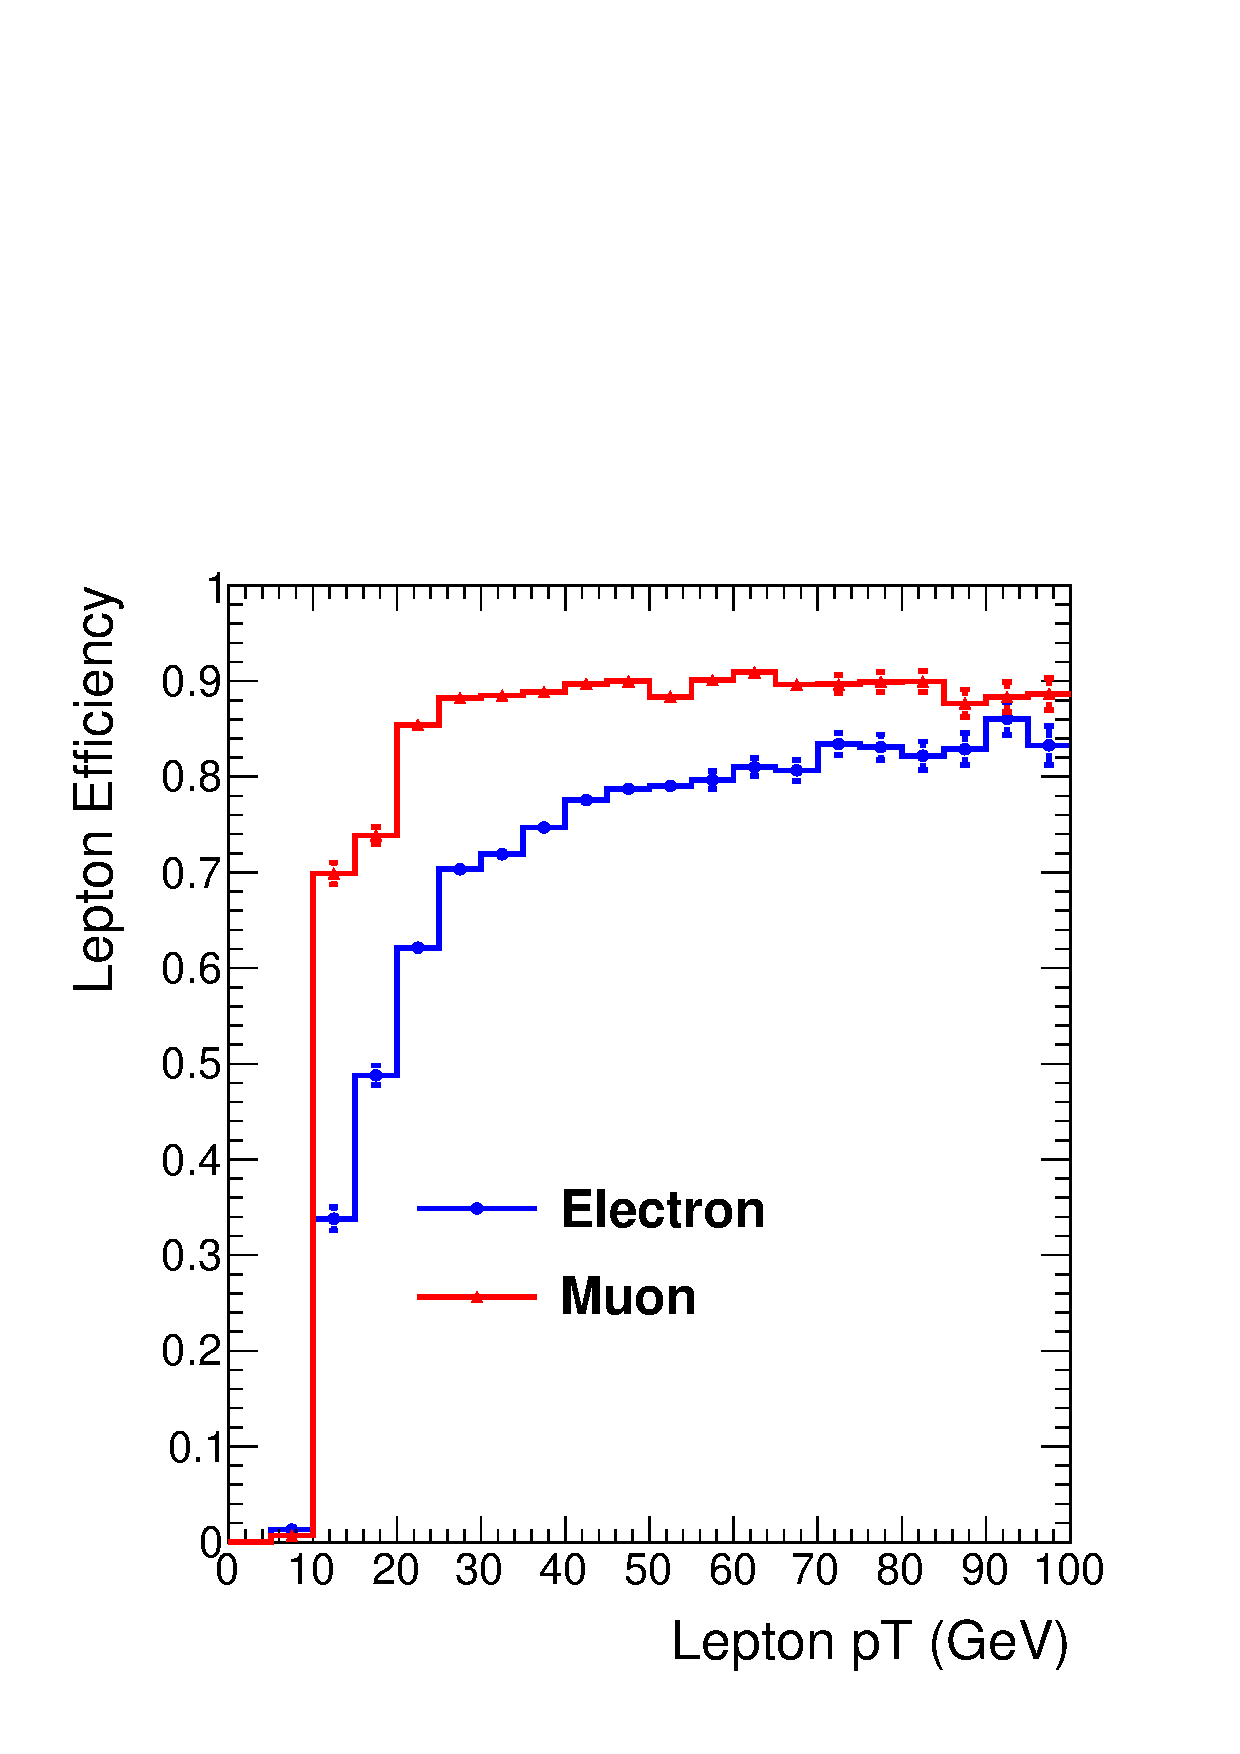
\includegraphics[width=0.4\textwidth]{figures/lepton_eff_Pt.pdf}\\
%\caption{{\bf this needs to be updated for the ZZ sample, especially with the pT 30/20 selection..}Lepton efficiency as a function of the lepton $\eta$ (left) and $\pt$ (right) extracted 
%from the $\ZZ$ Monte Carlo.}
%\label{fig:lepeff_gen}
%\end{center}
%\end{figure}
%%%%%%%%%%%%%%%%%%%%%%%%%%%%%%


%\subsection{{\bf $k_T$} Function}
One final complication that must be considered is the boost of the initial state.
In the leading order Matrix Element calculation there is no initial state radiation. 
%The initial state partons collide head-on and the system has no transverse boost. 
To account for the transverse recoil and thus improve the performance of our discriminant
on data, we integrate over the possible values of the system boost $k_{T}(k_{x},k_{y})$. 
The $k_T$ model is extracted from Monte Carlo for each process separately. 
In this case, we do not apply the dynamic event-by-event NLO reweighting procedure. 
%Figure~\ref{fig:zzboost} shows the distribution of $k_T$ for $\hzz$ and 
%the non-resonant $\ZZ$ processes.  


%%%%%%%%%%%%%%%%%%%%%%%%%%%%%%
%\begin{figure}[!htbp]
%\begin{center}
%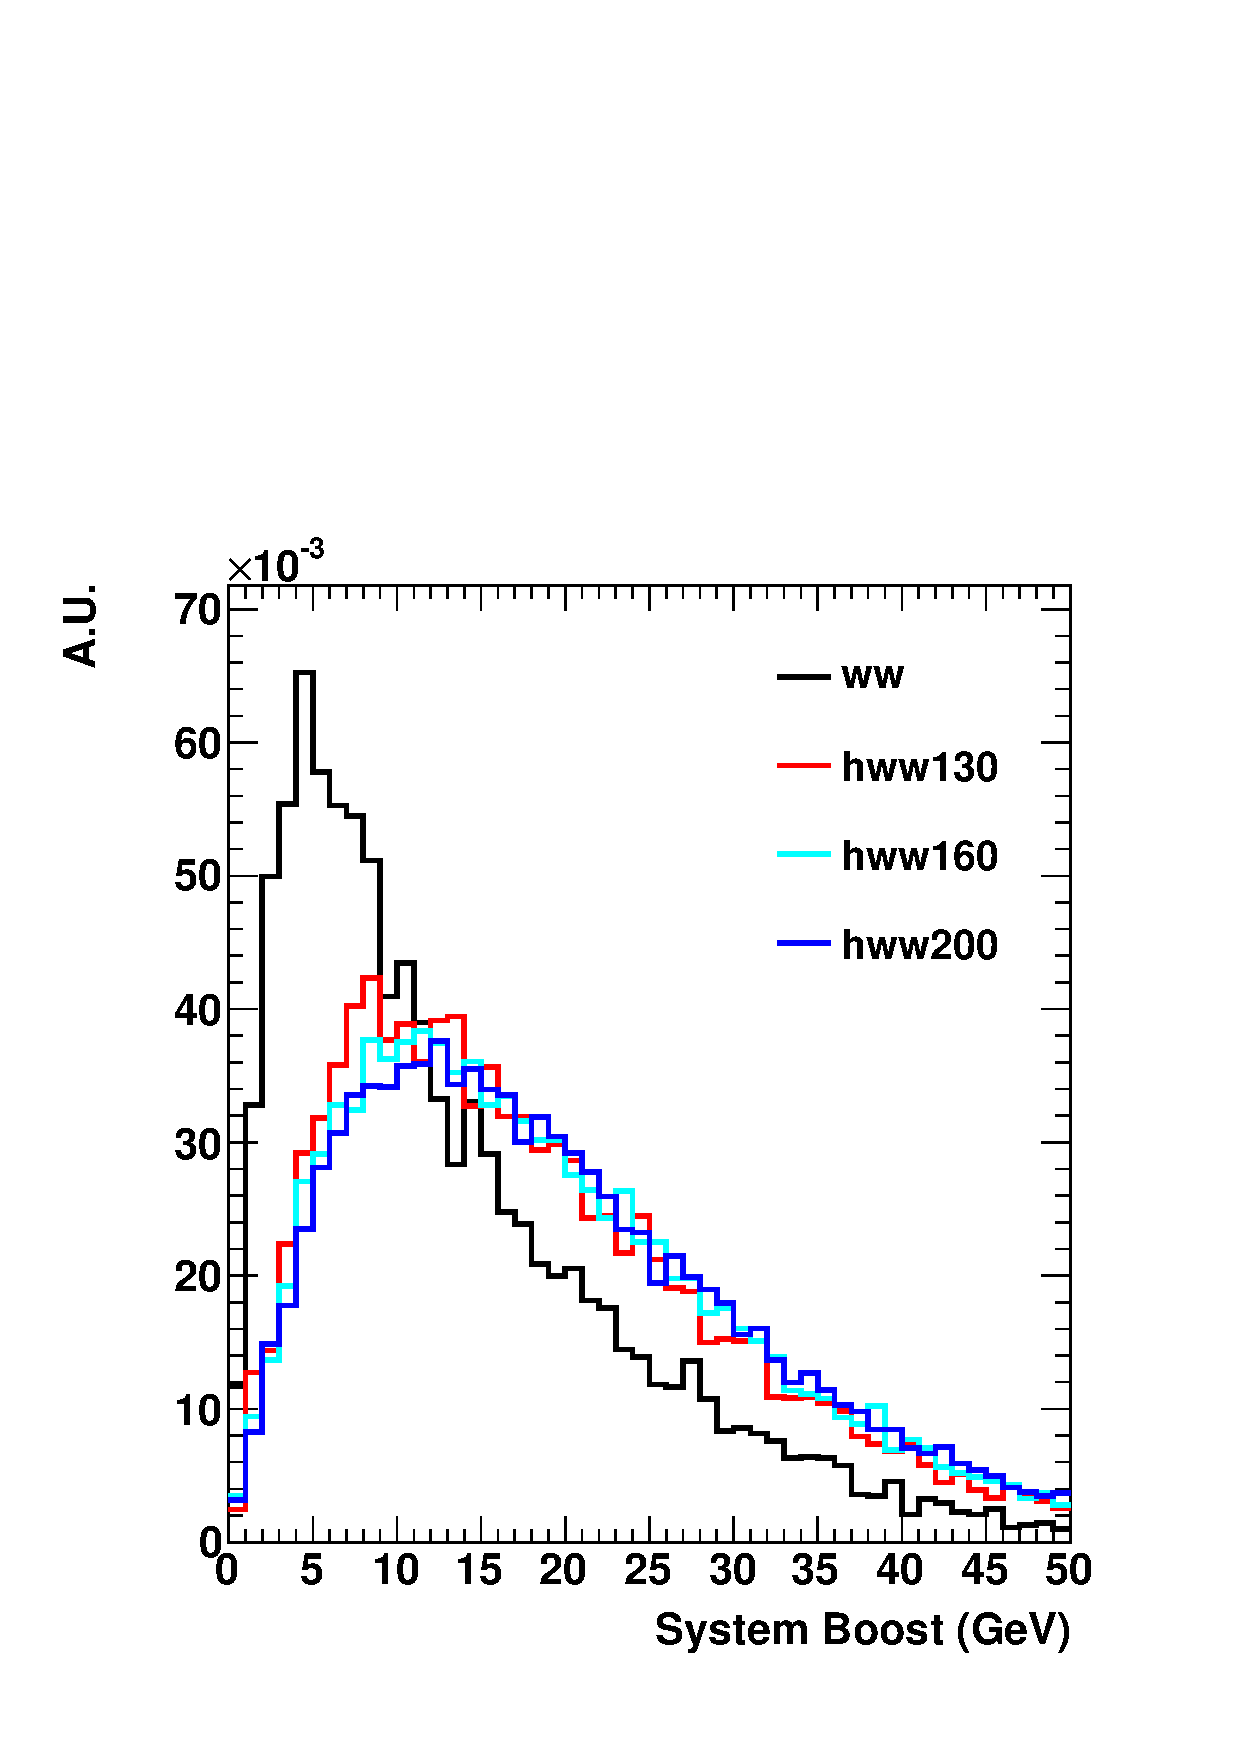
\includegraphics[width=0.5\textwidth]{figures/boost.pdf}
%\caption{{\bf This needs to be replaced with the ones from hzz properly...}The transverse boost of the $WW$ system for $ZZ$ production and $\hzz$ at 3 different Higgs masses.}
%\label{fig:zzboost}
%\end{center}
%\end{figure}
%%%%%%%%%%%%%%%%%%%%%%%%%%%%%%


\subsubsection{$\hzz$ Likelihood Ratio Discriminator}
Event probabilities, calculated as described above, are used to construct 
a likelihood ratio discriminant which we use in a one-dimensional template fit.  
The discriminator is defined as :
\begin{equation}
\label{eqn:LR}
LR = \frac { P_s} { P_s + \sum_i C_i k_{bi} P_{bi}},
\end{equation}
where $P_s$ is the probability for the signal, $P_{bi}$ is the probability for background
process $i$, and
$k_{bi}$ is the expected fractional contribution of background $i$,
satisfying the sum $\sum k_{bi} =1$, 
and $C_i$ is a constant which can be optimized for the best sensitivity independently for each 
Higgs mass hypothesis. 
Because signal events are expected to have $P_s>P_b$ and vice-versa for background events, 
the value of $LR$ is close to one for signal and zero for background processes.
The calculation of $P_s$ is a function of Higgs mass, so the likelihood ratio
shape depends on $m_H$. This is true for both signal and background templates of $LR$. 
%Figure~\ref{fig:lrstacks} shows the likelihood ratio distributions for $m_H$~=~130, 160, and 200 $\GeVcc$, 
%corresponding to 1~$\ifb$. 
%Note that the backgrounds peak near $LR~=~0$ while the signal peaks near $LR~=~1$. 
%%%%%%%%%%%%%%%%%%%%%%%%%%%%%%
%\begin{figure}[!hbtp]
%\centering
%\subfigure[]{
%\centering
%\label{subfig:lr_hm130}
%%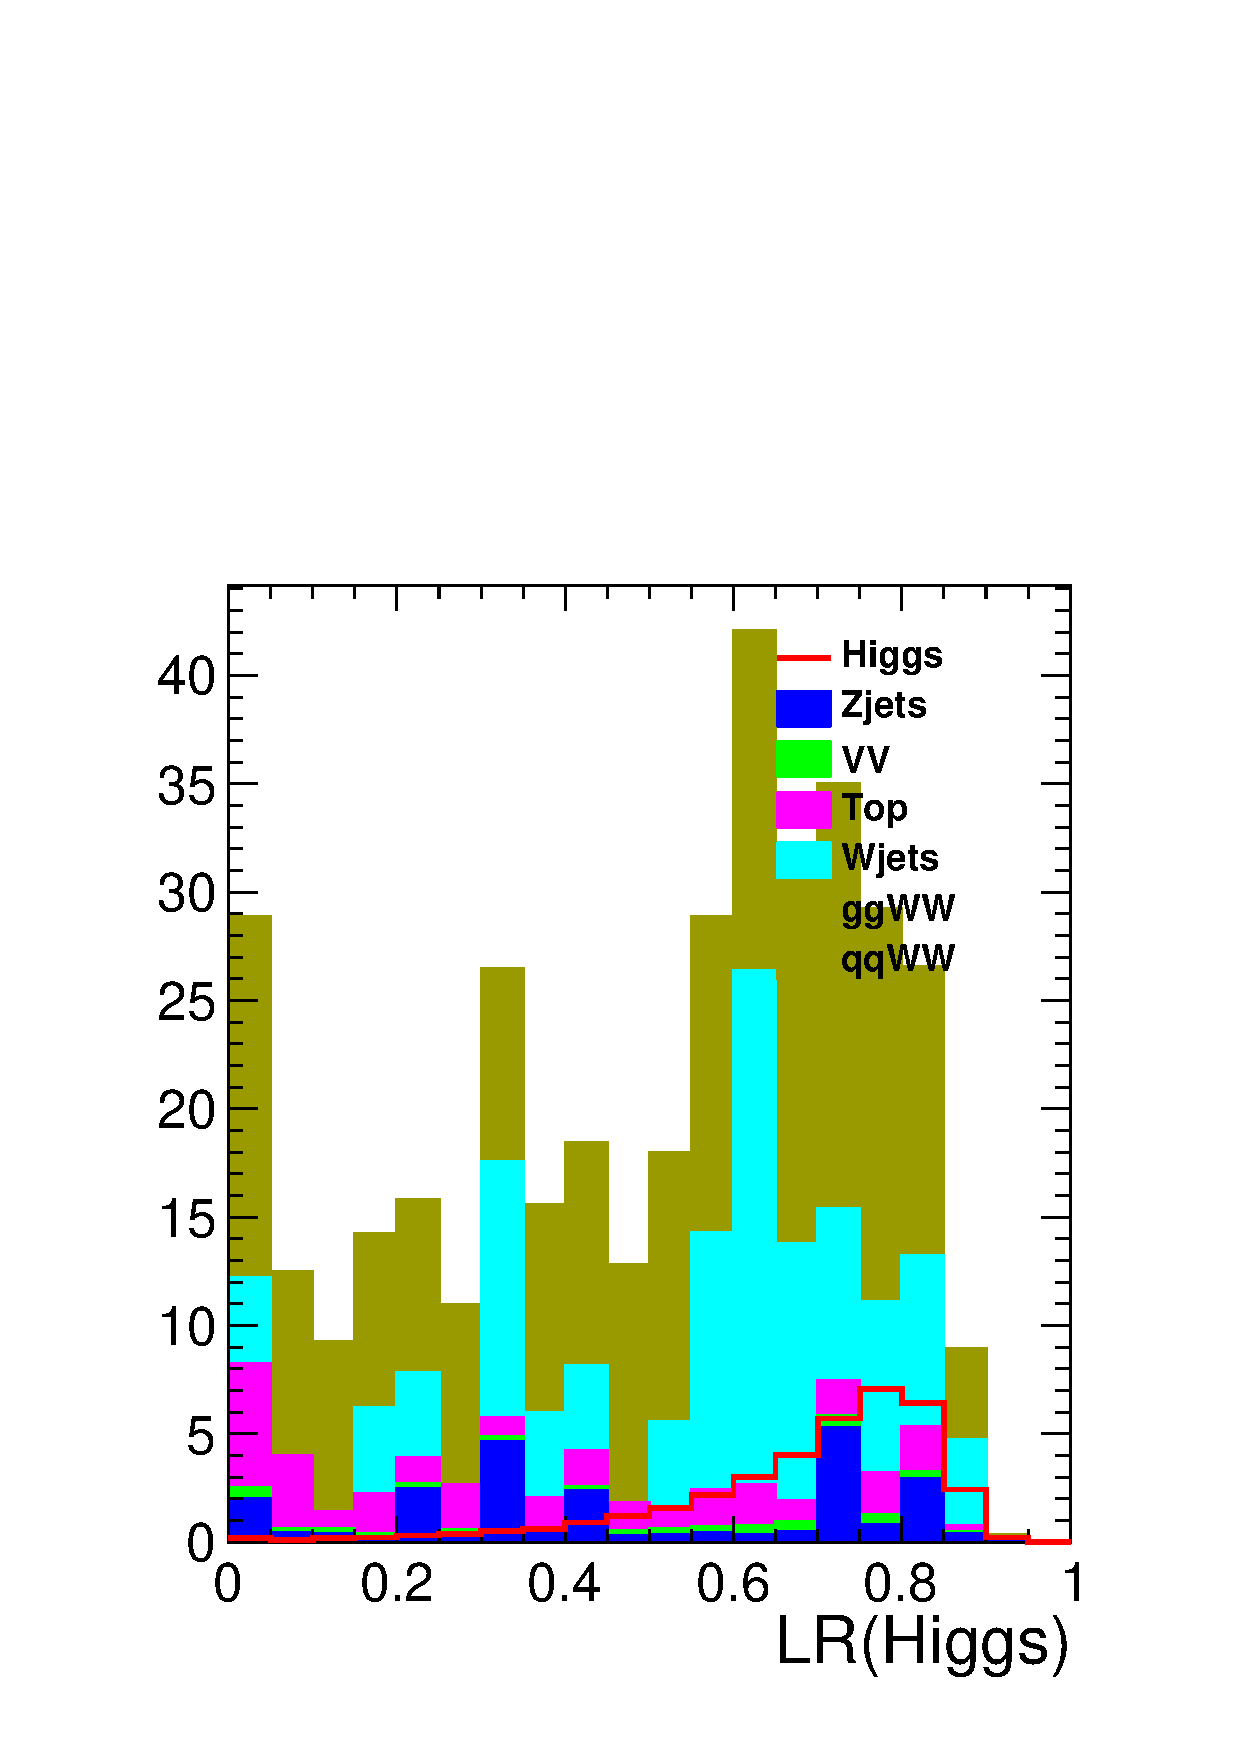
\includegraphics[width=.32\textwidth]{figures/hww130_LR.pdf}}
%}
%\caption{The matrix element output LR distribution after \ZZ\ pre-selection $m_H$=250 $\GeVcc$ 
%\subref{subfig:lr_hm130} in the 0-jet bin.}
%\label{fig:lrstacks}
%\end{figure}
%%%%%%%%%%%%%%%%%%%%%%%%%%%%%%

It is important to note that because the $LR$ distribution is calculated the same way for data, 
signal and backgrounds, the fact that we use a LO Matrix Element and make certain 
approximations in the analytic calculation may result in less than optimal sensitivity 
but are not expected to introduce any significant bias. 
This is because we apply the same method to calculate the differential 
cross sections for both the data and the simulated background samples.
We validate the matrix method by estimating the $\WZ/\ZZ$ cross-sections
shown in Appendix~\ref{app:zzxsec_me}. 

%Distributions of Higgs Likelihood Ratio for 3 test mass hypothesis are shown in 
%Fig.~\ref{fig:histo_me_250_5fb}-\ref{fig:histo_me_600_5fb}\fixme. 

%\begin{figure}[!ht]
%\begin{center}
%   \subfigure[]{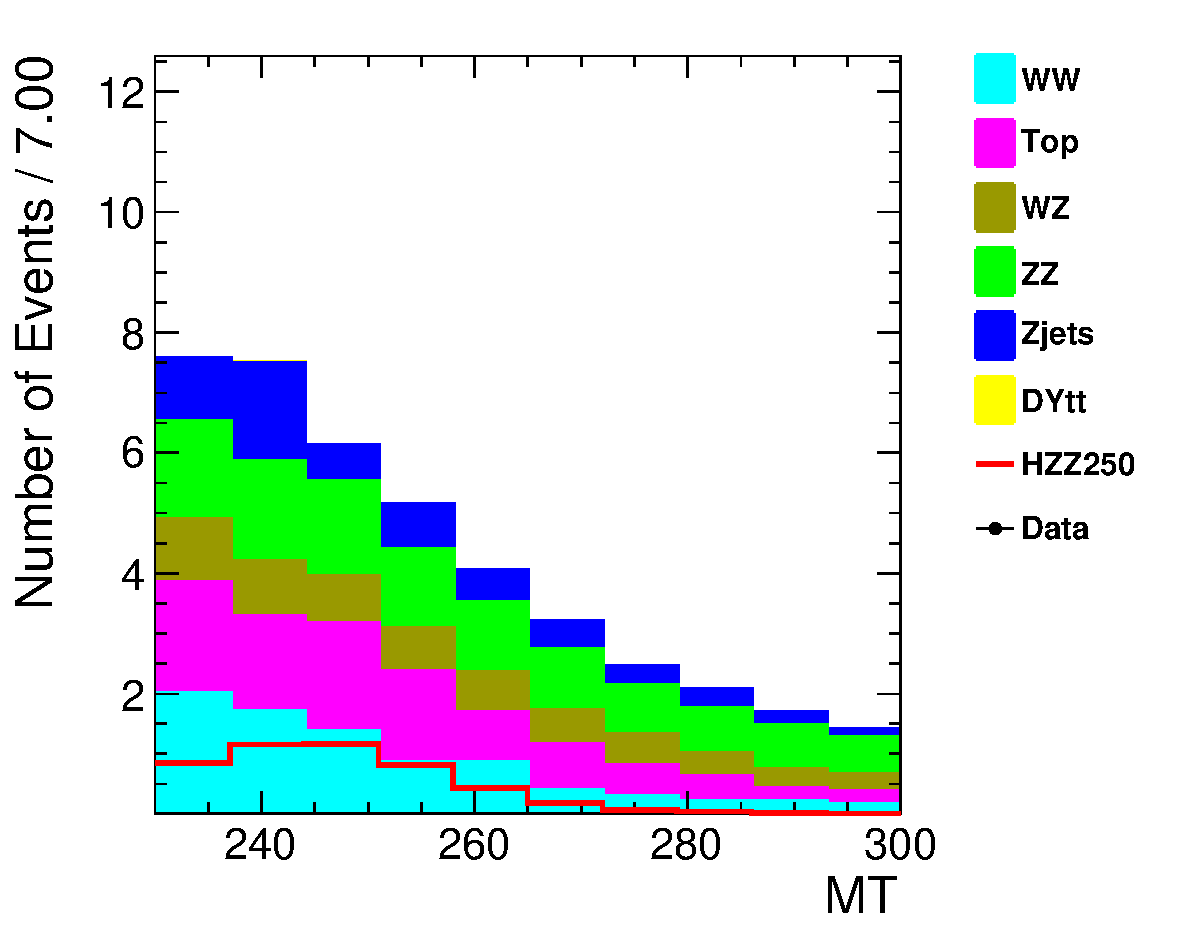
\includegraphics[width=0.4\textwidth,angle=0]{figures/MT_mH250_ee_stack_lin.pdf}} 
%   \subfigure[]{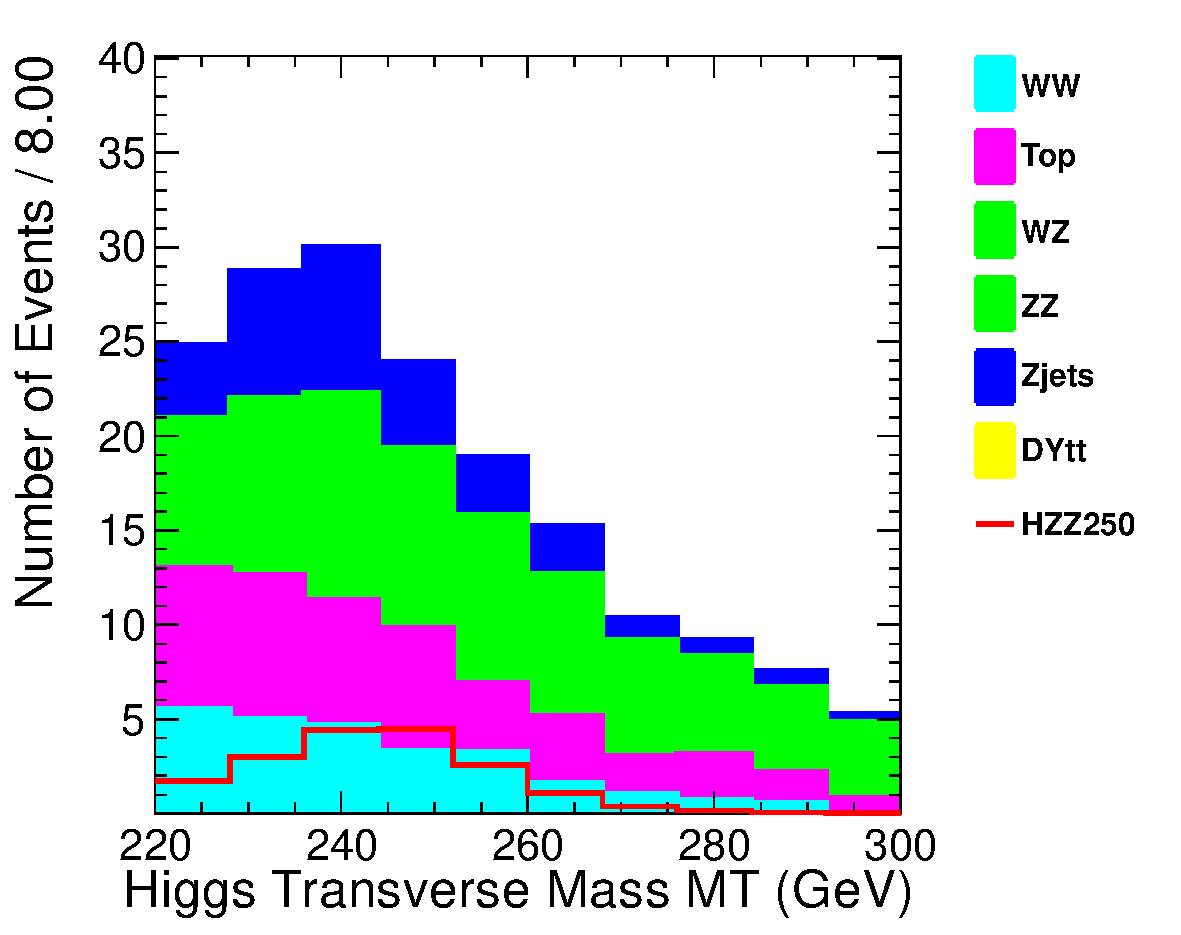
\includegraphics[width=0.4\textwidth,angle=0]{figures/MT_mH250_mm_stack_lin.pdf}} \\ 
%   \caption{The matrix element output distribution for Higgs signal and background events 
%for \mHi=250 $\GeVcc$ in ee (a) and $\mu\mu$ final state (b) after the Higgs dependent selections. 
%The distributions are normalized to 5~\ifb, with the background scaled by the data-to-mc ratios derived using 2.1~\ifb data. }
%   \label{fig:histo_me_250_5fb}
%\end{center}
%\end{figure}

%\begin{figure}[!ht]
%\begin{center}
%   \subfigure[]{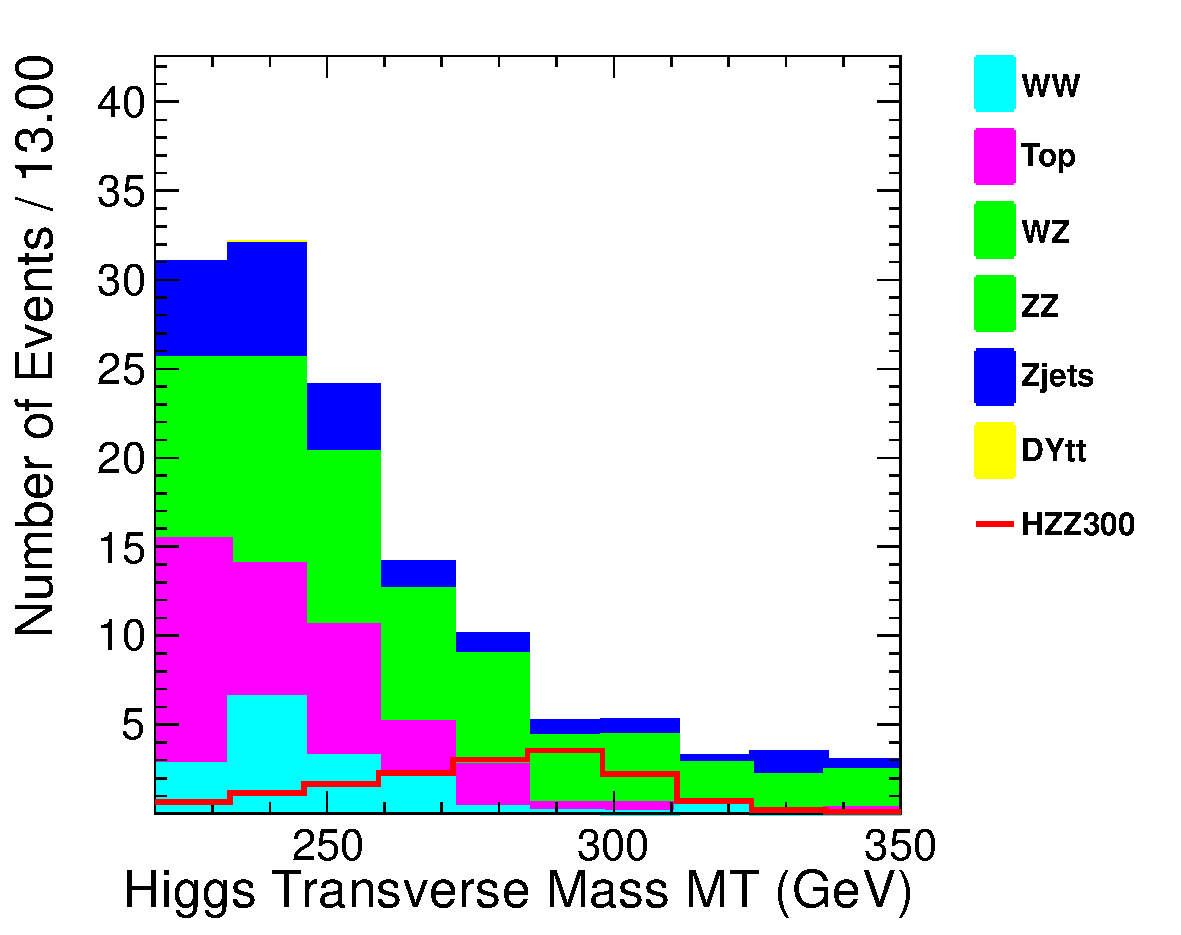
\includegraphics[width=0.4\textwidth,angle=0]{figures/MT_mH300_ee_stack_lin.pdf}} 
%   \subfigure[]{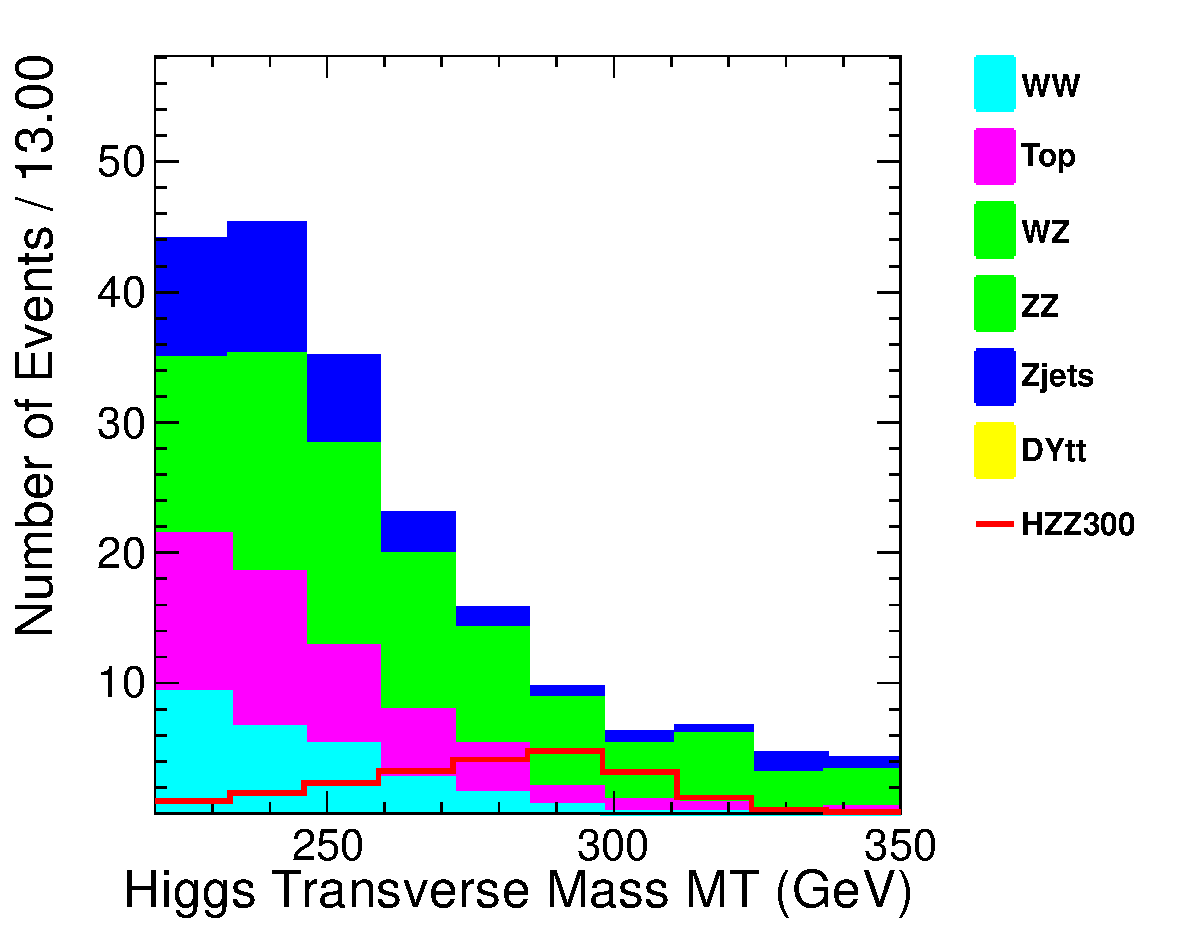
\includegraphics[width=0.4\textwidth,angle=0]{figures/MT_mH300_mm_stack_lin.pdf}} \\ 
%   \caption{The matrix element output distribution for Higgs signal and background events 
%for \mHi=300 $\GeVcc$ in ee (a) and $\mu\mu$ final state (b) after the Higgs dependent selections. 
%The distributions are normalized to 5~\ifb, with the background scaled by the data-to-mc ratios derived using 2.1~\ifb data. }
%   \label{fig:histo_me_300_5fb}
%\end{center}
%\end{figure}

%\begin{figure}[!ht]
%\begin{center}
%   \subfigure[]{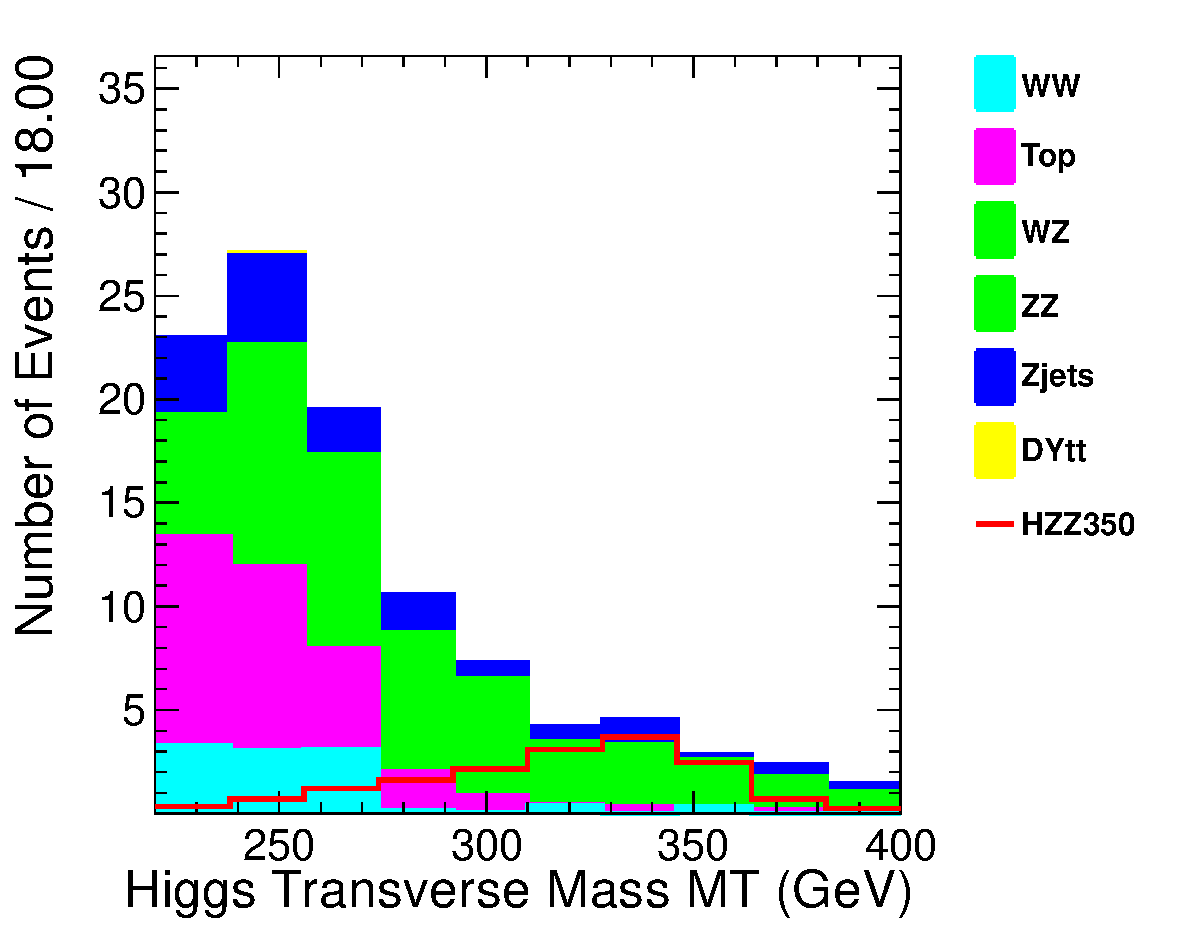
\includegraphics[width=0.4\textwidth,angle=0]{figures/MT_mH350_ee_stack_lin.pdf}} 
%   \subfigure[]{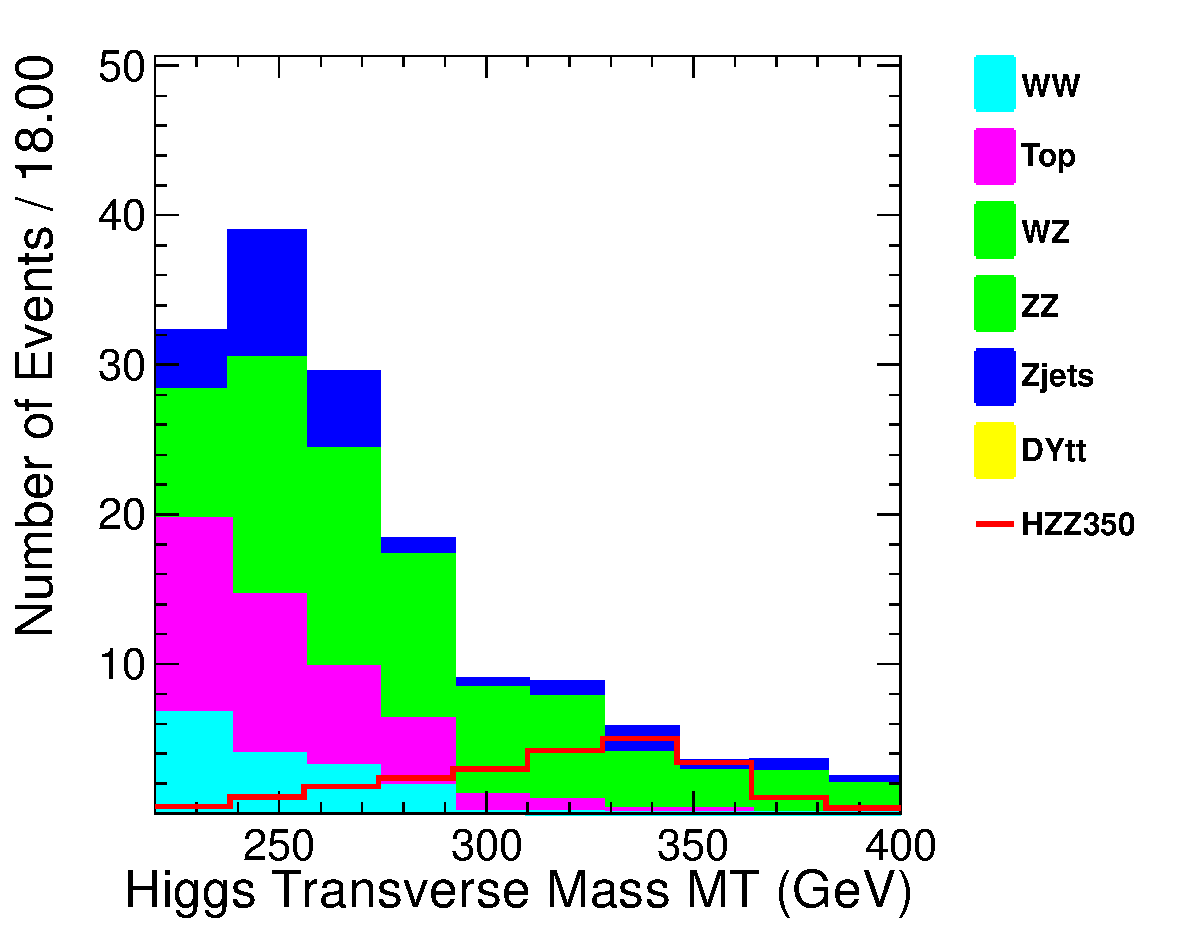
\includegraphics[width=0.4\textwidth,angle=0]{figures/MT_mH350_mm_stack_lin.pdf}} \\ 
%   \caption{The matrix element output distribution for Higgs signal and background events 
%for \mHi=350 $\GeVcc$ in ee (a) and $\mu\mu$ final state (b) after the Higgs dependent selections. 
%The distributions are normalized to 5~\ifb, with the background scaled by the data-to-mc ratios derived using 2.1~\ifb data. }
%   \label{fig:histo_me_350_5fb}
%\end{center}
%\end{figure}

%\begin{figure}[!ht]
%\begin{center}
%   \subfigure[]{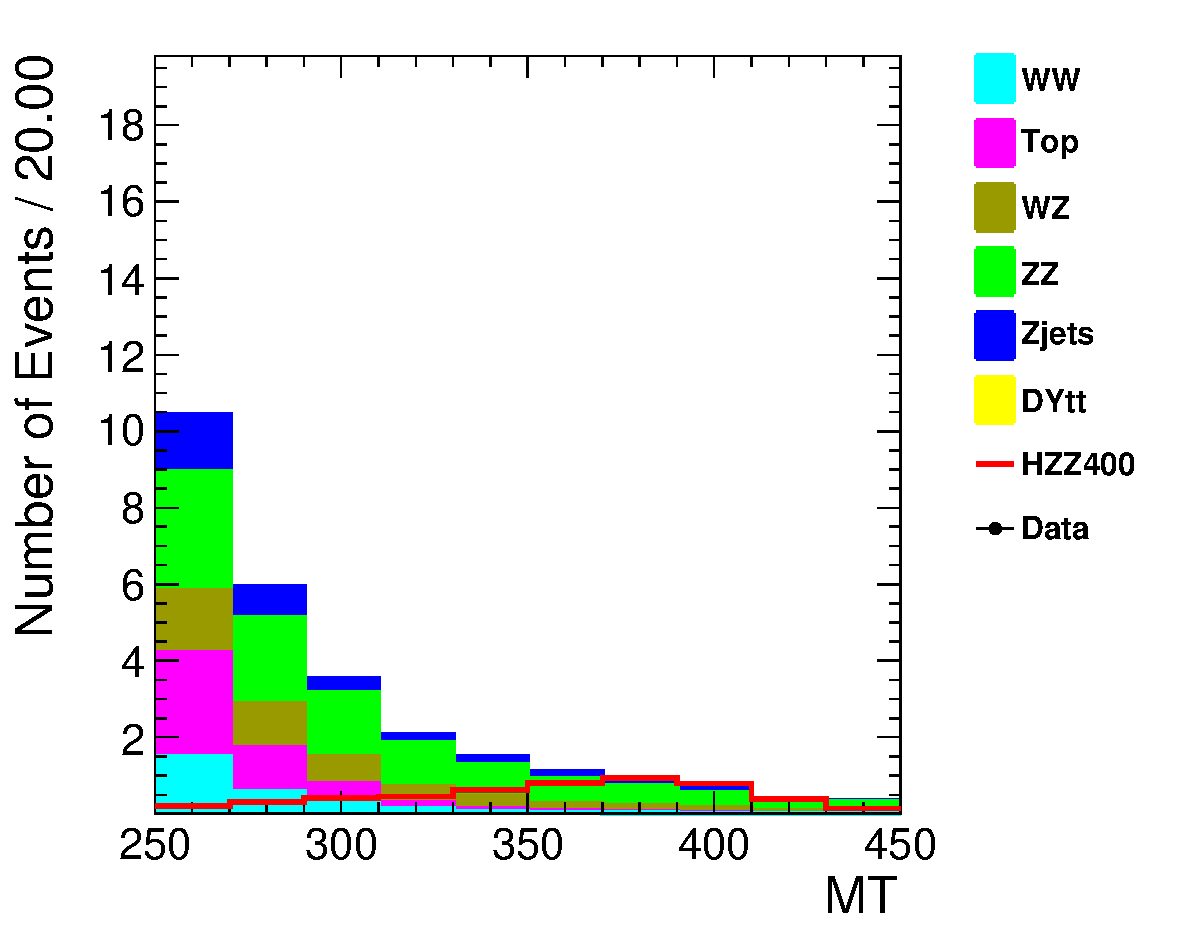
\includegraphics[width=0.4\textwidth,angle=0]{figures/MT_mH400_ee_stack_lin.pdf}} 
%   \subfigure[]{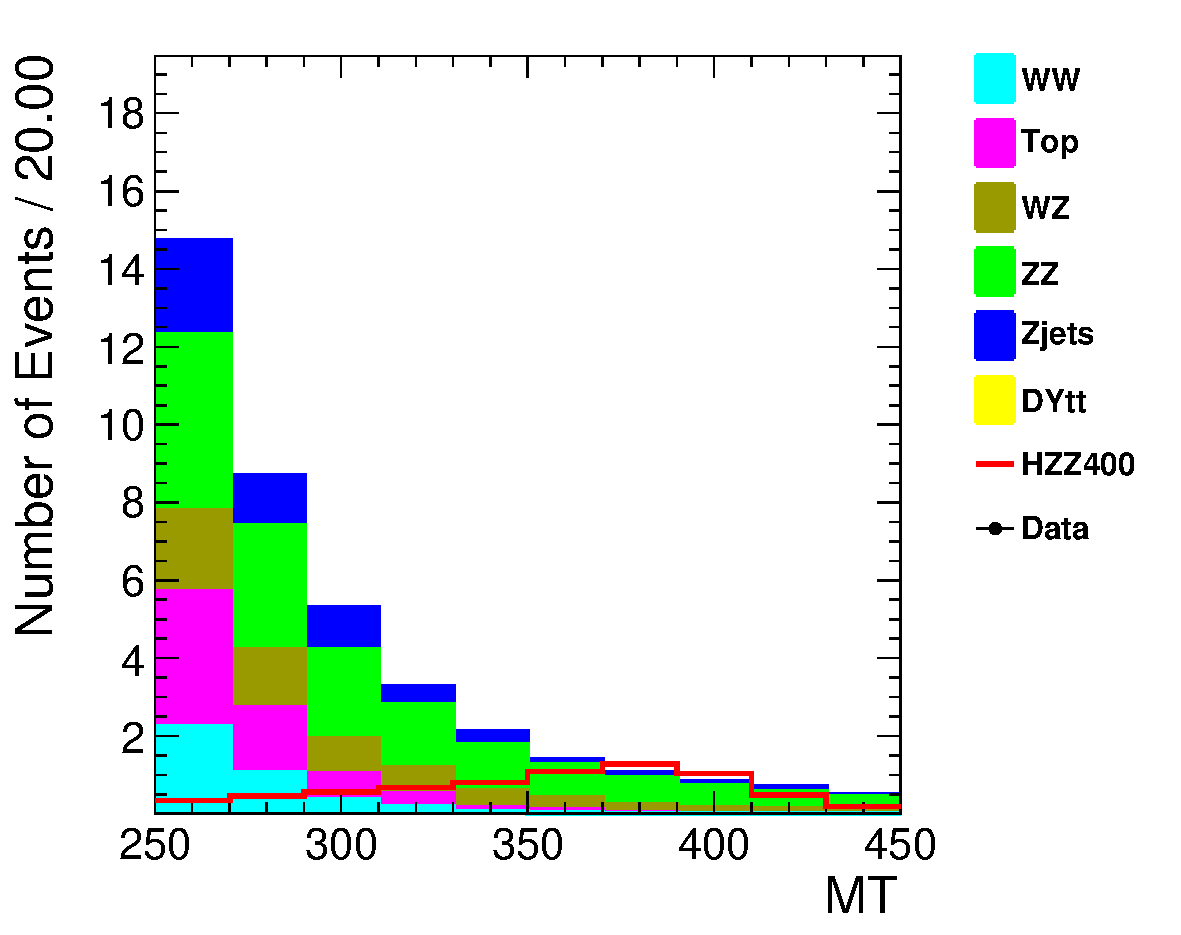
\includegraphics[width=0.4\textwidth,angle=0]{figures/MT_mH400_mm_stack_lin.pdf}} \\ 
%   \caption{The matrix element output distribution for Higgs signal and background events 
%for \mHi=400 $\GeVcc$ in ee (a) and $\mu\mu$ final state (b) after the Higgs dependent selections. 
%The distributions are normalized to 5~\ifb, with the background scaled by the data-to-mc ratios derived using 2.1~\ifb data. }
%   \label{fig:histo_me_400_5fb}
%\end{center}
%\end{figure}


%\begin{figure}[!ht]
%\begin{center}
%   \subfigure[]{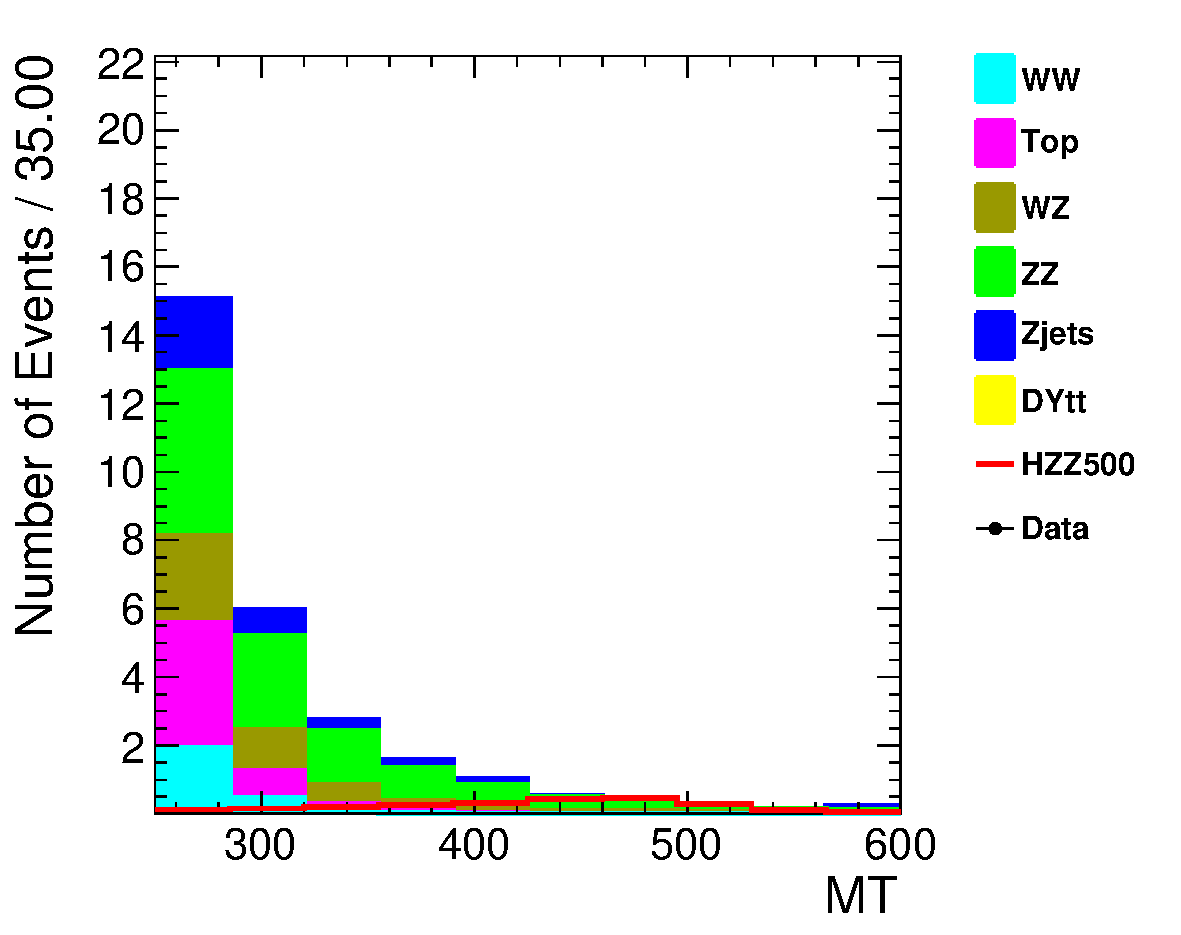
\includegraphics[width=0.4\textwidth,angle=0]{figures/MT_mH500_ee_stack_lin.pdf}} 
%   \subfigure[]{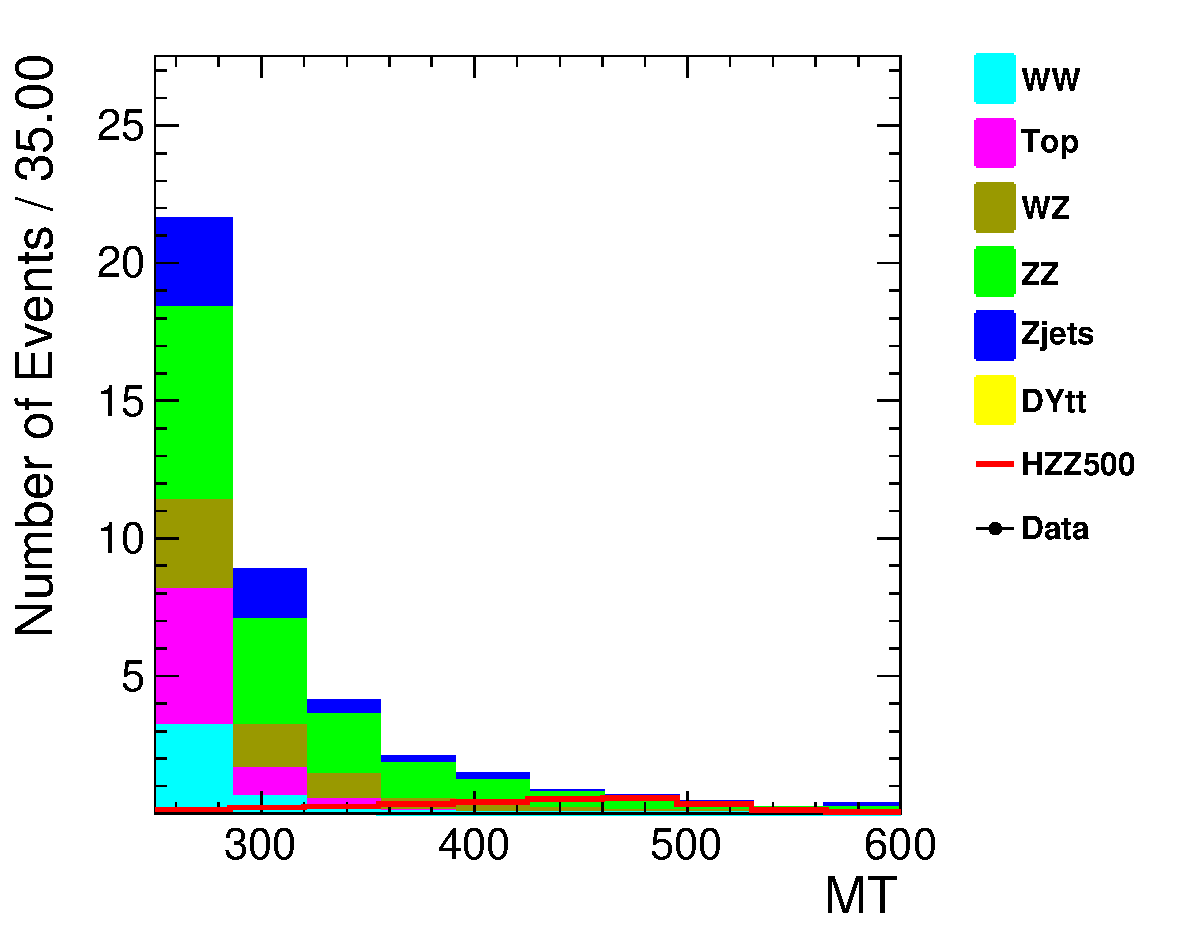
\includegraphics[width=0.4\textwidth,angle=0]{figures/MT_mH500_mm_stack_lin.pdf}} \\ 
%   \caption{The matrix element output distribution for Higgs signal and background events 
%for \mHi=500 $\GeVcc$ in ee (a) and $\mu\mu$ final state (b) after the Higgs dependent selections. 
%The distributions are normalized to 5~\ifb, with the background scaled by the data-to-mc ratios derived using 2.1~\ifb data. }
%   \label{fig:histo_me_500_5fb}
%\end{center}
%\end{figure}

%\begin{figure}[!ht]
%\begin{center}
%   \subfigure[]{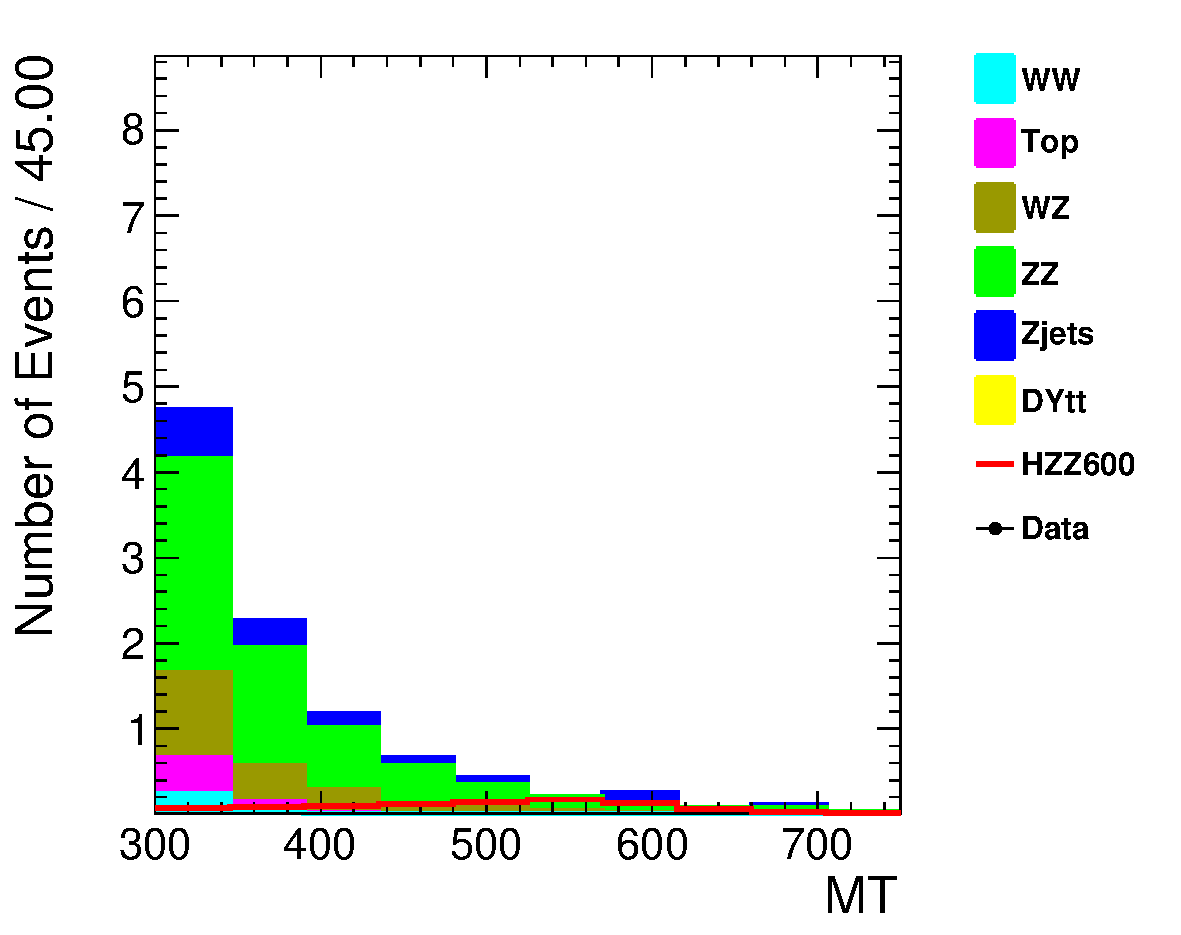
\includegraphics[width=0.4\textwidth,angle=0]{figures/MT_mH600_ee_stack_lin.pdf}} 
%   \subfigure[]{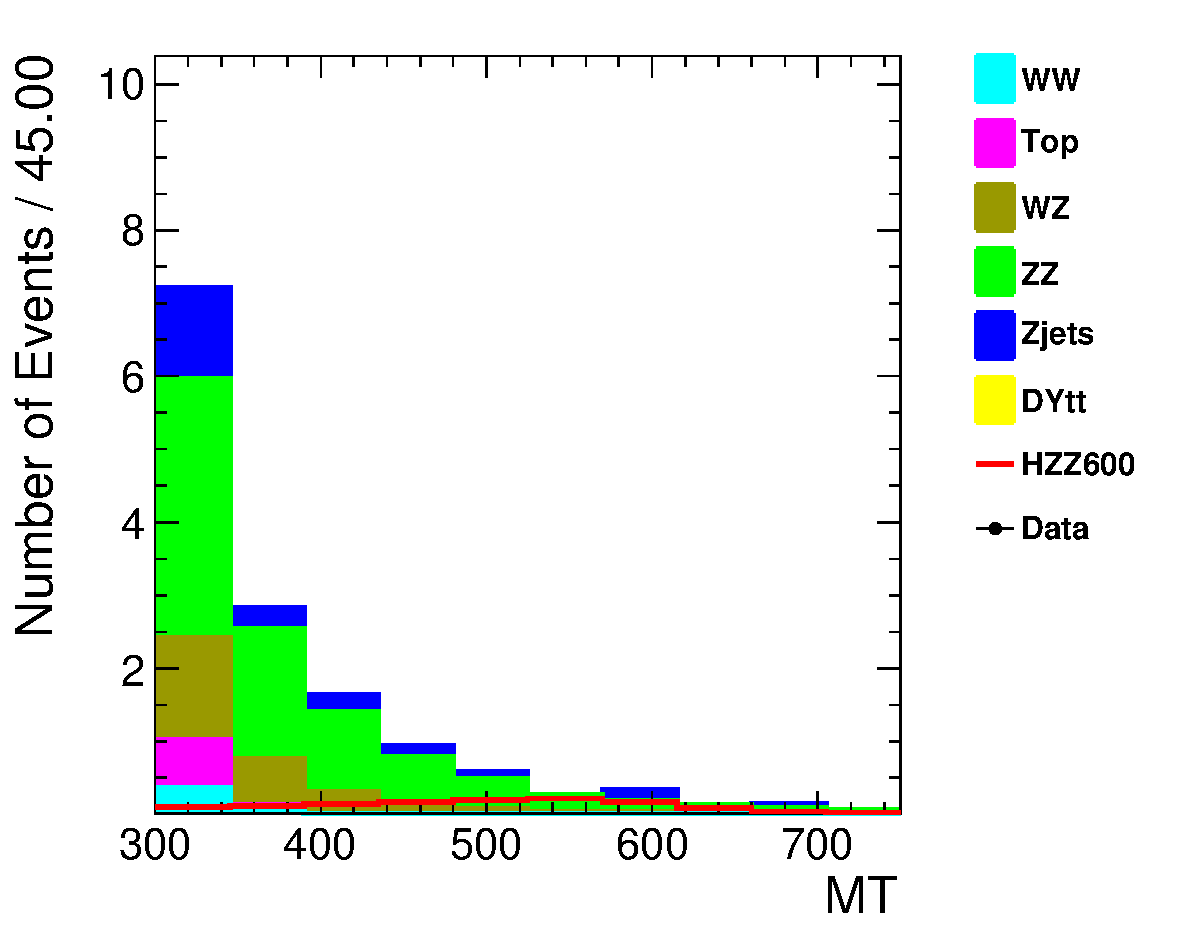
\includegraphics[width=0.4\textwidth,angle=0]{figures/MT_mH600_mm_stack_lin.pdf}} \\ 
%   \caption{The matrix element output distribution for Higgs signal and background events 
%for \mHi=600 $\GeVcc$ in ee (a) and $\mu\mu$ final state (b) after the Higgs dependent selections. 
%The distributions are normalized to 5~\ifb, with the background scaled by the data-to-mc ratios derived using 2.1~\ifb data. }
%   \label{fig:histo_me_600_5fb}
%\end{center}
%\end{figure}


%%%%%%%%%%%%%%%%%%%%%%%%%%%%%%
%\begin{figure}[!htbp]
%\begin{center}
%\subfigure[250 GeV]{\label{subfig:250GeV}
%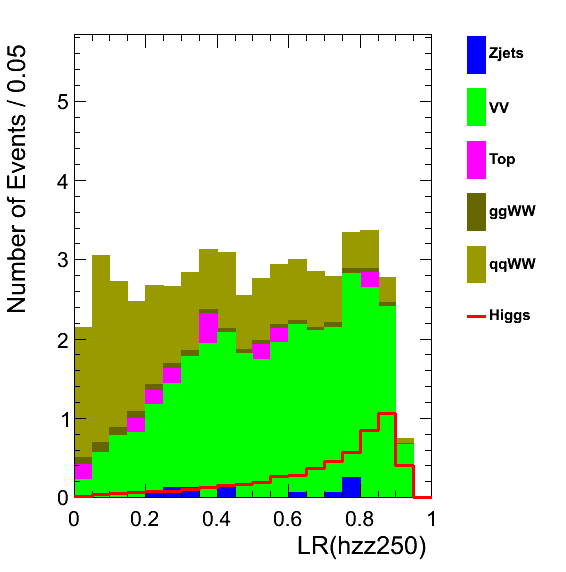
\includegraphics[width=0.3\textwidth]{figures/hzz250_LR.png}}
%\subfigure[300 GeV]{\label{subfig:300GeV}
%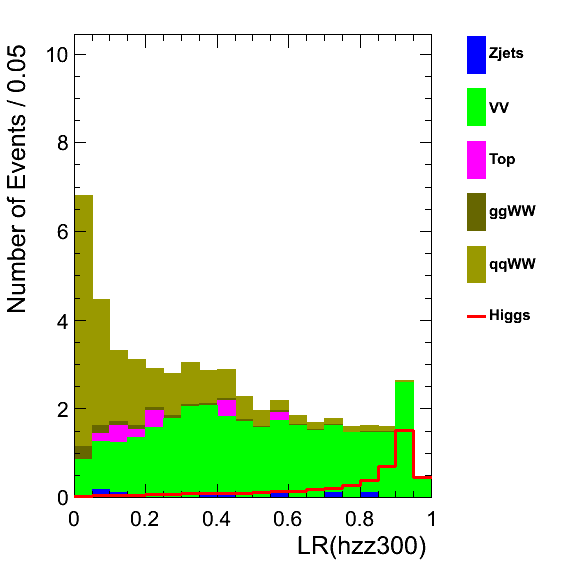
\includegraphics[width=0.3\textwidth]{figures/hzz300_LR.png}}
%\subfigure[400 GeV]{\label{subfig:400GeV}
%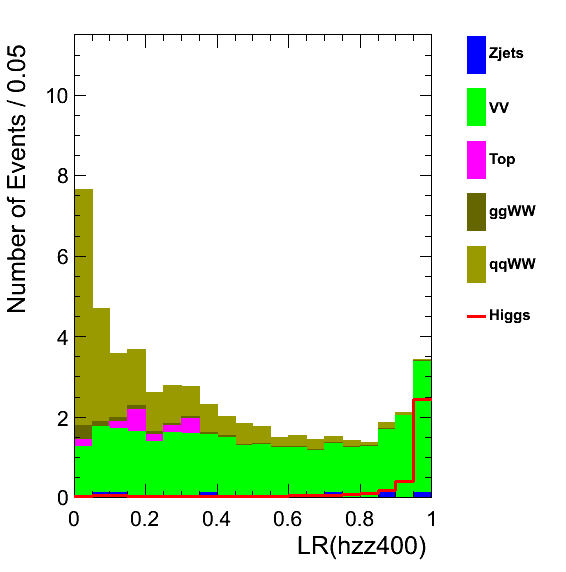
\includegraphics[width=0.3\textwidth]{figures/hzz400_LR.png}}
%\caption{$LR_{HZZ}$ in 1092 pb$^{-1}$ for expected backgrounds and signal.}
%\label{fig:lrhzz}
%\end{center}
%\end{figure}
%%%%%%%%%%%%%%%%%%%%%%%%%%%%%%


